\documentclass[../TDM3_courbe_app.tex]{subfiles}%

\begin{document}
\section[s]"3"{Anneau sur une tige en rotation}

\noindent
\enonce{%
	\noindent
	\begin{minipage}{0.70\linewidth}
		On considère un petit anneau M de masse $m$ considéré comme ponctuel, soumis
		à la pesanteur et susceptible de se déplacer sans frottement le long d'une
		tige OA horizontale dans le plan ($x$O$y$), de longueur $\ell$, effectuant
		des mouvements de rotation caractérisés par une vitesse angulaire $\w$
		constante autour d'un axe fixe vertical $\D$ passant par son extrémité O. Le
		référentiel lié au laboratoire est considéré comme galiléen. On considère~:
		\bigbreak
		\begin{itemize}
			\item le repère cartésien $(\Or,\ex,\ey,\ez)$ fixe dans le référentiel
			      du laboratoire et associé aux axes $x$, $y$ et $z$~;
			\item la base cylindrique locale $(\er,\et,\ez)$ associée au point M.
		\end{itemize}
		\bigbreak
	\end{minipage}
	\hfill
	\begin{minipage}{0.25\linewidth}
		\begin{center}
			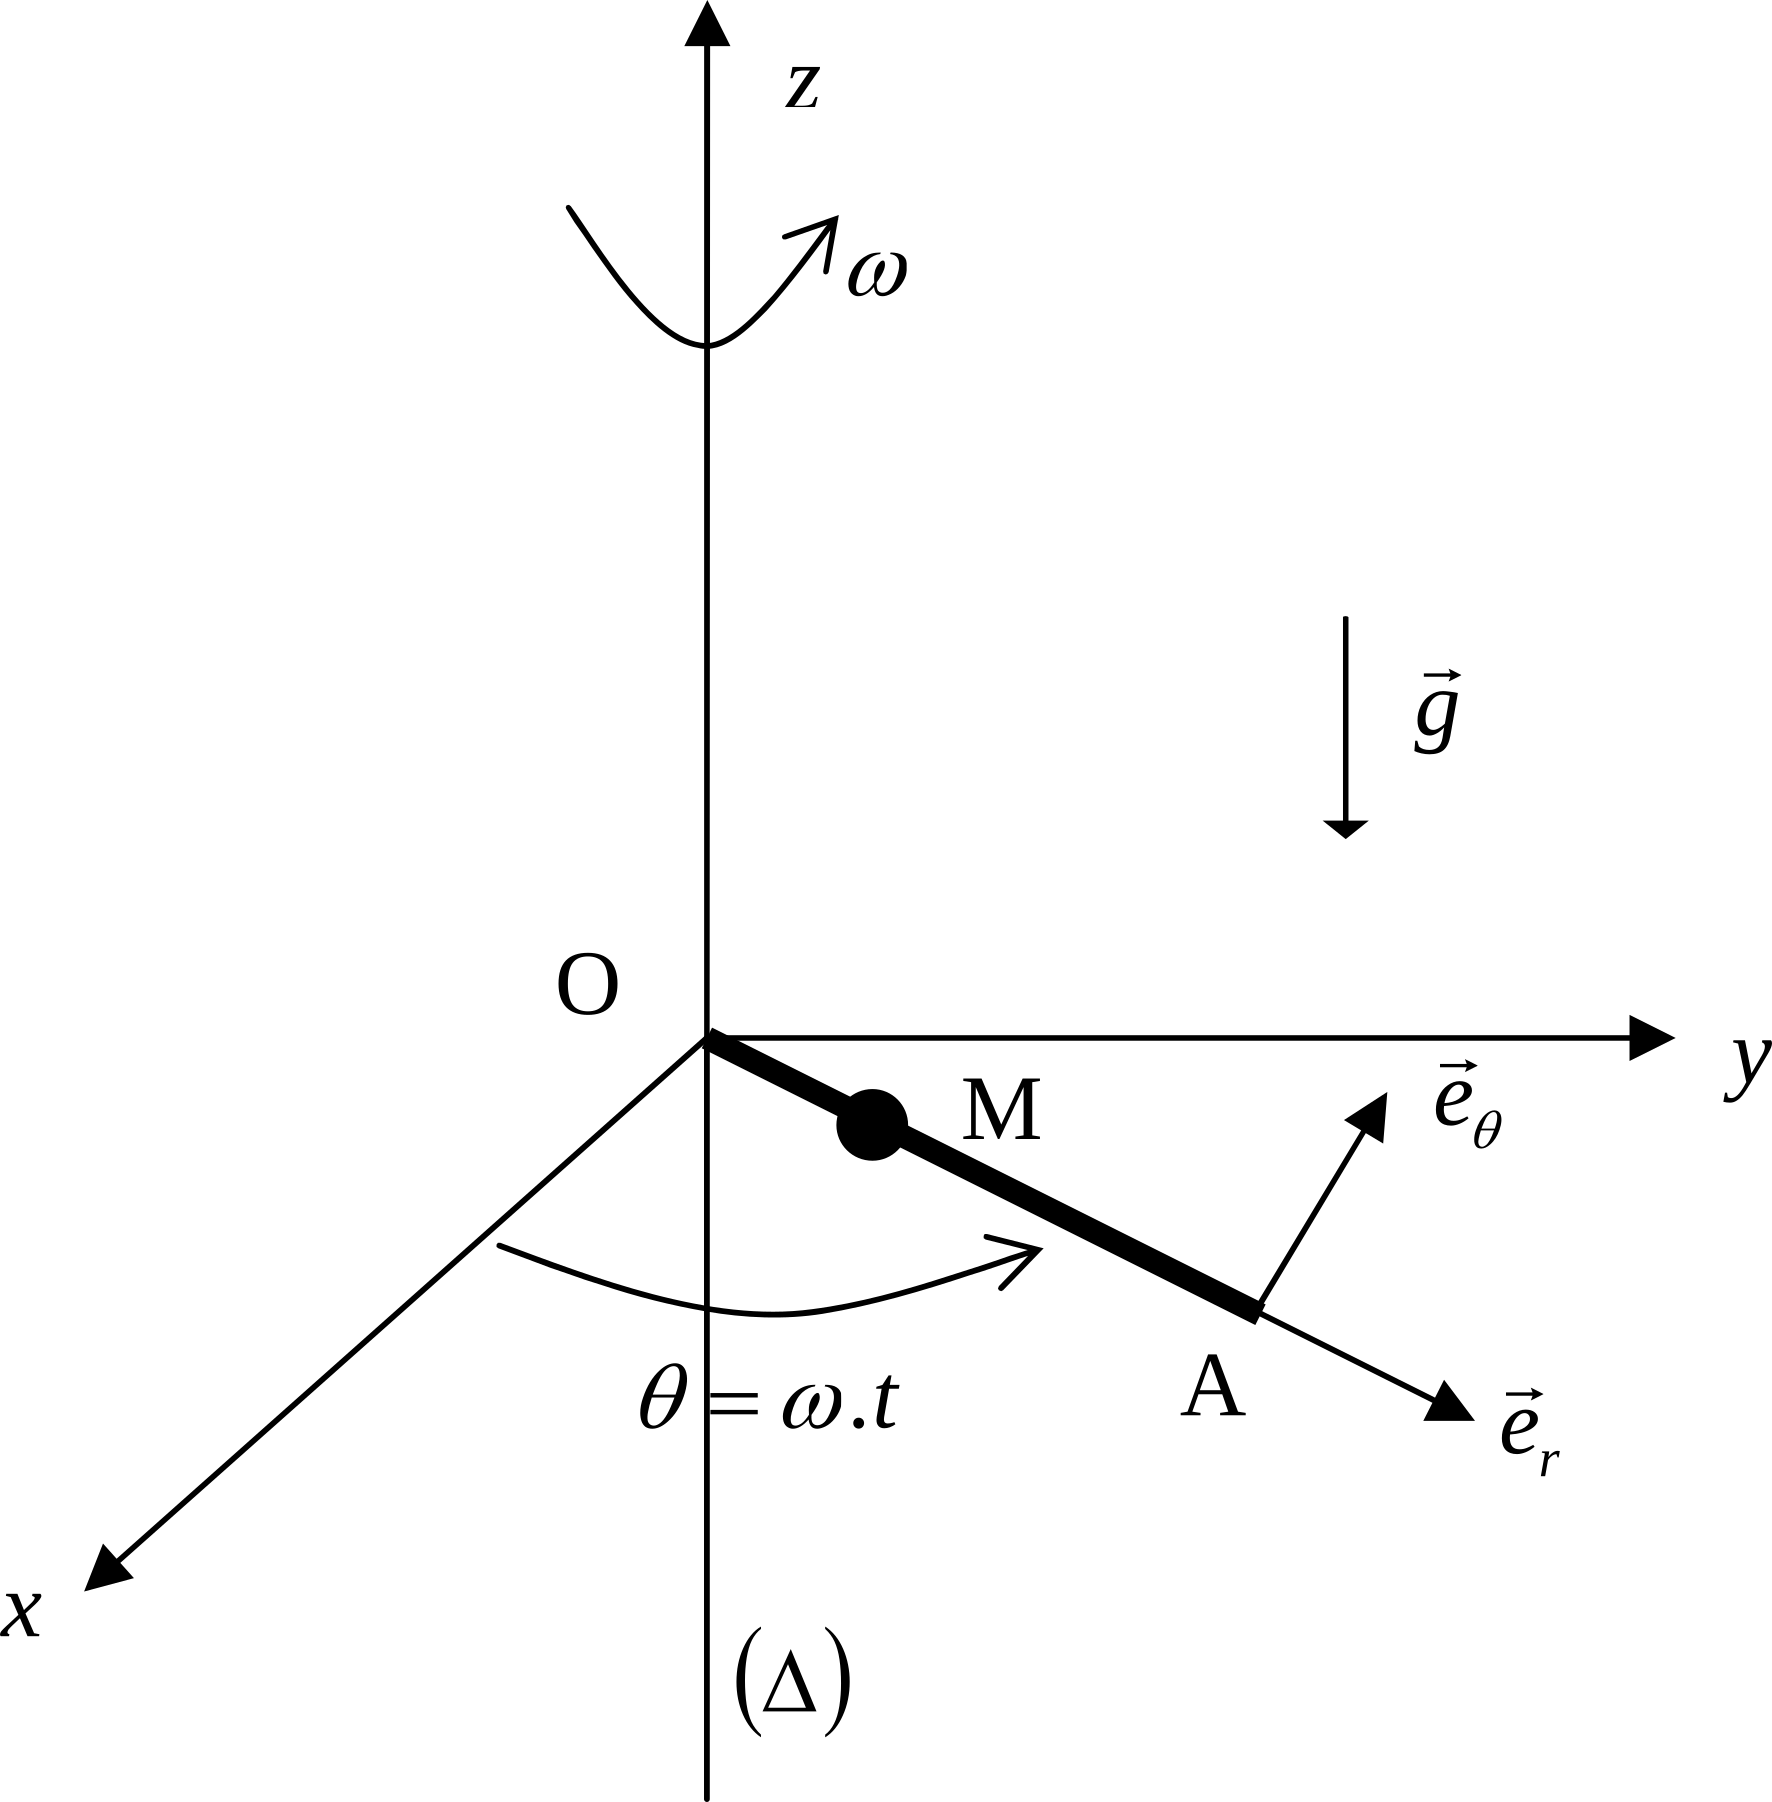
\includegraphics[width=\linewidth]{anneau_tige_rot-plain}
		\end{center}
	\end{minipage}
	L'anneau est libéré sans vitesse initiale par rapport à la tige, à une
	distance $r_0$ du point O (avec $r_0 < \ell$). On repère la position de
	l'anneau sur la tige par la distance $r = \OMr$ entre le point O et l'anneau
	M.
}%

\QR{%
	Faire un bilan des forces agissant sur l'anneau en les projetant dans
	la base $(\er,\et,\ez)$. En appliquant le
	principe fondamental de la dynamique, établir l'équation différentielle
	vérifiée par $r(t)$.
}{%
	\begin{minipage}[t]{0.60\linewidth}
		\begin{itemize}[label=$\diamond$, leftmargin=10pt]
			\item[b]{Système}~: \{anneau\} point matériel M de masse $m$
			\item[b]{Référentiel}~: terrestre supposé galiléen
			\item[b]{Repère}~: cylindrique $(\Or,\er,\et,\ez)$
			\item[b]{Repérage}~:
			      \begin{align*}
				      \OM & = r\er                                        \\
				      \vf & = \rp\er + r\tp\et                            \\
				          & = \rp\er + r\w\et                             \\
				      \af & = \rpp\er + \rp\tp\et + \rp\w\et - r\w^2\er +
				      \underbracket[0.4pt]{\of}_{\dot{\w}=0}              \\
				          & = (\rpp -r\w^2)\er +2r\w\et
			      \end{align*}
		\end{itemize}
	\end{minipage}
	\hfill
	\begin{minipage}[t]{0.35\linewidth}
		~
		%\vspace*{6cm}
		\begin{center}
			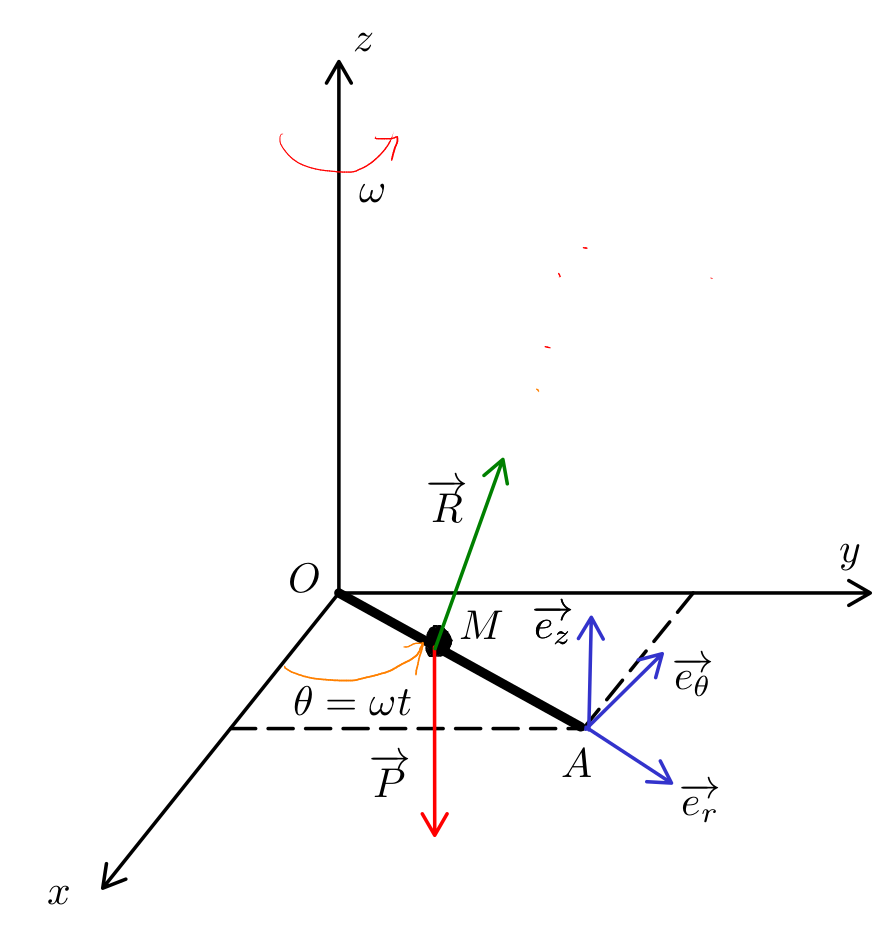
\includegraphics[scale=.18]{tige_rot_corr}
		\end{center}
	\end{minipage}
	\begin{itemize}[label=$\diamond$, leftmargin=10pt]
		\item[b]{Conditions initiales}~:
		      \[
			      r(0) = r_0
			      \qet
			      \vf(0) = \of \Ra \rp(0) = 0
		      \]
		\item[b]{BDF}~: pas de frottements donc pas de composante sur $\er$~:
		      \[
			      \begin{array}{ll}
				      \textbf{Poids}            & \Pf = m\gf = -mg\ez     \\
				      \textbf{Réaction support} & \Rf = R_\th\et + R_z\ez
			      \end{array}
		      \]
		\item[b]{PFD}~:
		      \begin{gather*}
			      m\af = \Pf + \Rf
			      \Lra
			      \left\{
			      \begin{aligned}
				      m(\rpp-r\w^2) & = 0         \\
				      2m\rp\w       & = R_\th     \\
				      0             & = -mg + R_z
			      \end{aligned}
			      \right.
		      \end{gather*}
		      \begin{empheq}[box=\fbox, left=\Lra\empheqlbrace]{align}
			      \label{eq:tigerota}
			      \Aboxed{
				      \rpp - \w r &= 0
			      }\\
			      \label{eq:tigerotb}
			      R_\th &= 2m\rp\w\\
			      \label{eq:tigerotc}
			      R_z &= mg
		      \end{empheq}
	\end{itemize}
}
\QR{%
	Intégrer cette équation différentielle en prenant en compte les
	conditions initiales définies précédemment, et déterminer la solution
	$r(t)$ en fonction de $r_0$, $\w$ et $t$.
}{%
	On résout~\eqref{eq:tigerota} avec l'équation caractéristique~:
	\begin{align*}
		\rpp -\w^2r & = 0
		\\\Ra
		s^2 - \w^2  & = 0
		\\\Lra
		s^2         & = \w^2
		\\\Lra
		\Aboxed{s   & = \pm\w}
	\end{align*}
	On a donc des solutions de la forme
	\begin{gather*}
		r(t) = A\exr^{\wt} + B\exr^{-\wt}
		\shortintertext{Or, avec les CI}~:
		\begin{aligned}
			r(0)        & = r_0
			\\\Lra
			\Aboxed{r_0 & = A+B}
		\end{aligned}
		\shortintertext{et}
		\begin{aligned}
			\rp(0)    & = 0
			\\\Lra
			0         & = A\w -B\w
			\\\Lra
			\Aboxed{A & = B}
		\end{aligned}
		\shortintertext{Soit}
		\\
		\boxed{A = B = \frac{r_0}{2}}
		\Ra
		\boxed{r(t) = \frac{r_0}{2}(\exr^{\wt} + \exr^{-\wt}) =
			r_0\cosh(\wt)}
	\end{gather*}
}
\QR{%
	Exprimer les composantes de la réaction $\Rf$ de la tige sur M dans la
	base $(\er,\et,\ez)$ en fonction de $m$, $g$, $\rp$ et $\w$.
}{%
	On reprend~\eqref{eq:tigerotb} et~\eqref{eq:tigerotc} avec $\rp =
		\w r_0\sinh(\wt)$~:
	\[
		\boxed{
			\Rf = 2mr_0\w^2\sinh(\wt)\et + mg\ez
		}
	\]
}
\QR{%
	Déduire de la question 2 le temps $\tau$ que va mettre l'anneau pour
	quitter la tige. On exprimera $\tau$ en fonction de $r_0$, $\ell$ et
	$\w$.
}{%
	L'anneau quitte la tige en $\tau$ quand $r(\tau) = \ell$, soit
	\begin{gather*}
		\ell = r_0\cosh(\wt)
		\\\Lra
		\boxed{\tau = \frac{1}{\w}\acosh(\wt)}
	\end{gather*}
}
\end{document}
